\documentclass[10pt]{article}

\usepackage{amsmath}

\newcommand{\myvec}[1]{\ensuremath{\begin{pmatrix}#1\end{pmatrix}}}

\newcommand{\mydet}[1]{\ensuremath{\begin{vmatrix}#1\end{vmatrix}}}

\newcommand{\solution}{\noindent \textbf{Solution: }}

\providecommand{\brak}[1]{\ensuremath{\left(#1\right)}}

\providecommand{\norm}[1]{\left\lVert#1\right\rVert}
\usepackage{graphicx}
\usepackage{float}

\let\vec\mathbf
\title{Coordinate Geometry}
\author{K.Hritik (kottahritik@sriprakshschools.com)}

\begin{document}
\maketitle
\section*{10$^{th}$ Maths - Chapter 7}
This is Problem-9 from Exercise 7.2
\begin{enumerate}
\item Find the coordinates of the points which divide the line segment joining A (- 2, 2) and B (2, 8) into four equal parts.  \\
\solution \\
\
Given Data:A = \myvec{-2\\2}\\
           B = \myvec{2\\8}\\
\\To find:C,D,E = ?\\

   let,k=1 
Now, 
\begin{align}
C = \frac{A+kB}{k+1}\\
C = \frac{\myvec{-2\\2}+1\myvec{2\\8}}{(1+1)}\\
= \frac{\myvec{-2\\2}+\myvec{2\\8}}{2}\\
= \frac{\myvec{0\\10}}{2}\\
 = \myvec{0\\5}\\
C = (0,5)
\end{align}	
now, 
\begin{align}
D = \frac{A+kC}{k+1}\\
D = \frac{\myvec{-2\\2}+1\myvec{0\\5}}{(1+1)}\\
= \frac{\myvec{-2\\2}+\myvec{0\\5}}{2}\\
= \frac{\myvec{-2\\7}}{2}\\
= \myvec{-1\\\frac{7}{2}}\\
D = (-1,\frac{7}{2})
\end{align}
Similarly,the third point 
\begin{align}
E = \frac{C+kB}{k+1}\\
E = \frac{\myvec{0\\5}+1\myvec{2\\8}}{(1+1)}\\
= \frac{\myvec{0\\5}+\myvec{2\\8}}{2}\\
= \frac{\myvec{2\\13}}{2}\\
 = \myvec{2\\\frac{13}{2}}\\
E = (2,\frac{13}{2})
\end{align}
therefore,the three points which divide AB into four equal parts are:\\
C = (0,5),
D = $(-1,\frac{7}{2})$,
E = $(2,\frac{13}{2})$
\end{enumerate}

\begin{figure}[H]
			\centering
			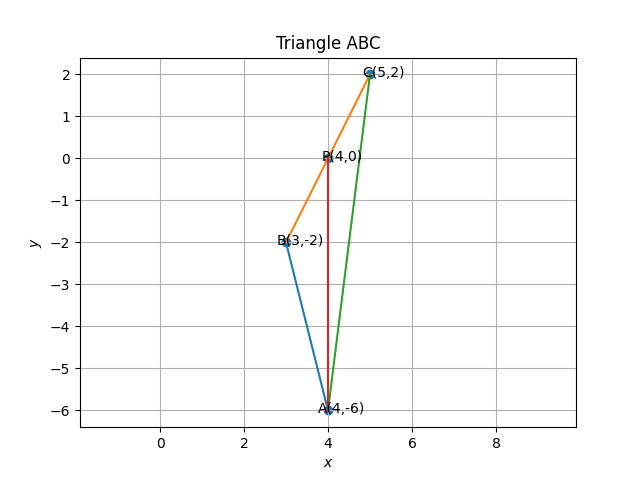
\includegraphics[width=\columnwidth]{figs/Figure_1.png}
			\caption{Line segment AB}
			\label{fig:3}
		\end{figure}
\end{document}
